% Presentation on Predator-Prey models
% 07.05.2020, Moritz Konarski, AUCA

%==============================================================================
% SETUP

\documentclass[hyperref={colorlinks,allcolors=black}]{beamer}

\mode<presentation>
{
  \usetheme{Goettingen}                     % set general look
  \usecolortheme{seahorse}                  % set color scheme
  \usefonttheme{serif}                      % set font to latex-like
  \setbeamertemplate{navigation symbols}{}
  \setbeamertemplate{caption}[numbered]
} 

\usepackage[english]{babel}
\usepackage[utf8]{inputenc}
\usepackage[T1]{fontenc}
\usepackage{amsmath}
\usepackage{amsfonts}
\usepackage{textcomp}
\usepackage{graphicx}
\graphicspath{{../graphics/}}
\usepackage{subfig}
\usepackage{wrapfig}
\usepackage{float}
\usepackage{caption}


\newcommand{\figref}[1]{\textsc{\figurename}~\ref{#1}}

\newcommand{\makefig}[4]{
\begin{figure}[#1]
    \captionsetup{justification=centering}
    \includegraphics[width=#2]{#3}
    \caption{#4}
    \label{fig:#3}
\end{figure}
}

\newcommand{\makewrapfig}[5]{
\begin{wrapfigure}{#1}{#2}
    \captionsetup{margin=10pt,justification=centering}
    \includegraphics[width=#3]{#4}
    \caption{#5}
    \label{fig:#4}
\end{wrapfigure}
}

\AtBeginSection[]{
    \begin{frame}
    \vfill
    \centering
    \begin{beamercolorbox}[sep=8pt,center,shadow=false,rounded=false]{title}
    \usebeamerfont{title}\insertsectionhead\par
    \end{beamercolorbox}
    \vfill
    \end{frame}
}

\setbeamertemplate{frametitle}[default][center]
\setbeamertemplate{bibliography item}{\insertbiblabel}

%==============================================================================
% PRESENTATION

%------------------------------------------------------------------------------
% GENERAL INFORMATION

\title[Predator-Prey Equations]{Predator-Prey Equations:\\Modeling Food Chains}
\author[M. Konarski]{Moritz M. Konarski}
\institute[AUCA]{Applied Mathematics Department \newline 
    American University of Central Asia}
\date{\today}

\begin{document}

\begin{frame}
  \titlepage
\end{frame}

\begin{frame}{Outline}
  \tableofcontents
\end{frame}

\section{Introduction}

\subsection{Background}

\begin{frame}{Background}
\begin{itemize}
\setlength\itemsep{1em}
    \item differential equations describing populations of predators and prey
    \item most famous are Lotka-Volterra equations
    \item derived by Alfred James Lotka (1880--1949) and Vito Volterra
        (1860--1940) \cite{hoppensteadt} in the 1920s
    \item Volterra observed fish, Lotka chemical reactions -- both are the same
        system \cite{hoppensteadt}
\end{itemize}
\end{frame}

\subsection[Equations]{Lotka-Volterra Equations}

\begin{frame}{Lotka-Volterra Equations}
\begin{itemize}
\setlength\itemsep{1em}
    \item simplest predator-prey equations
    \item parameters $a,b,c,d>0$, following \cite{chauvet}
\end{itemize}
\begin{equation}    
    \left\{\begin{aligned}
        &\frac{dx}{dt} = ax - bxy \quad &\text{Prey}\\
        &\frac{dy}{dt} = -cy +dxy \quad &\text{Predator}
    \end{aligned}\right.
    \label{eq:2s_system}
\end{equation}
\end{frame}

\subsection[Expanded Equations]{Expanded Lotka-Volterra Equations}

\begin{frame}{Expanded Lotka-Volterra Equations}
    \begin{itemize}
\setlength\itemsep{1em}
        \item expansion of \eqref{eq:2s_system}
        \item parameters $a,b,c,d,e,f,g>0$, following \cite{chauvet}
    \end{itemize}
\begin{equation}
    \left\{\begin{aligned}
        &\frac{dx}{dt} = ax - bxy              &\text{Prey}\\
        &\frac{dy}{dt} = -cy + dxy - eyz \quad &\text{Intermediate Predator}\\
        &\frac{dz}{dt} = -fz + gyz             &\text{Apex Predator}
    \end{aligned}\right.
    \label{eq:3s_system}
\end{equation}
\end{frame}

\subsection{Phase Planes}

\begin{frame}{Phase Planes}
    \begin{itemize}
\setlength\itemsep{1em}
        \item space where all points are solutions of a system like
            \eqref{eq:2s_system}
        \item moving points form trajectories
        \item stationary points are equilibria \cite{terman}
        \item example of pendulum in \figref{fig:example_phase_plane}
        \item give insights into equation without solving
    \end{itemize}
\end{frame}

\begin{frame}{Phase Planes - Example}
$x'=y$ and $y'=-\sin(x)$
    \makefig{h}{0.7\textheight}{example_phase_plane}{Phase plane of a pendulum with contour lines}
\end{frame}

\section{Two-Species Food Chain}

\begin{frame}{Two-Species Food Chain}
    \begin{itemize}
\setlength\itemsep{1em}
        \item standard Lotka-Volterra equations
        \item equivalent to \eqref{eq:3s_system} with $z=0$
        \item parameters $a=b=c=d=1$ chosen for simplicity
    \end{itemize}
\begin{equation}
    \left\{\begin{aligned}
        &\frac{dx}{dt} = x(1 - y) \quad &\text{Prey,}\\
        &\frac{dy}{dt} = y(x - 1) \quad &\text{Predator.}
    \end{aligned}\right.
    \label{eq:2s_example}
\end{equation}
\end{frame}

\begin{frame}{Phase Plane}
\begin{figure}[H]%
\subfloat[Phase plane]{
    {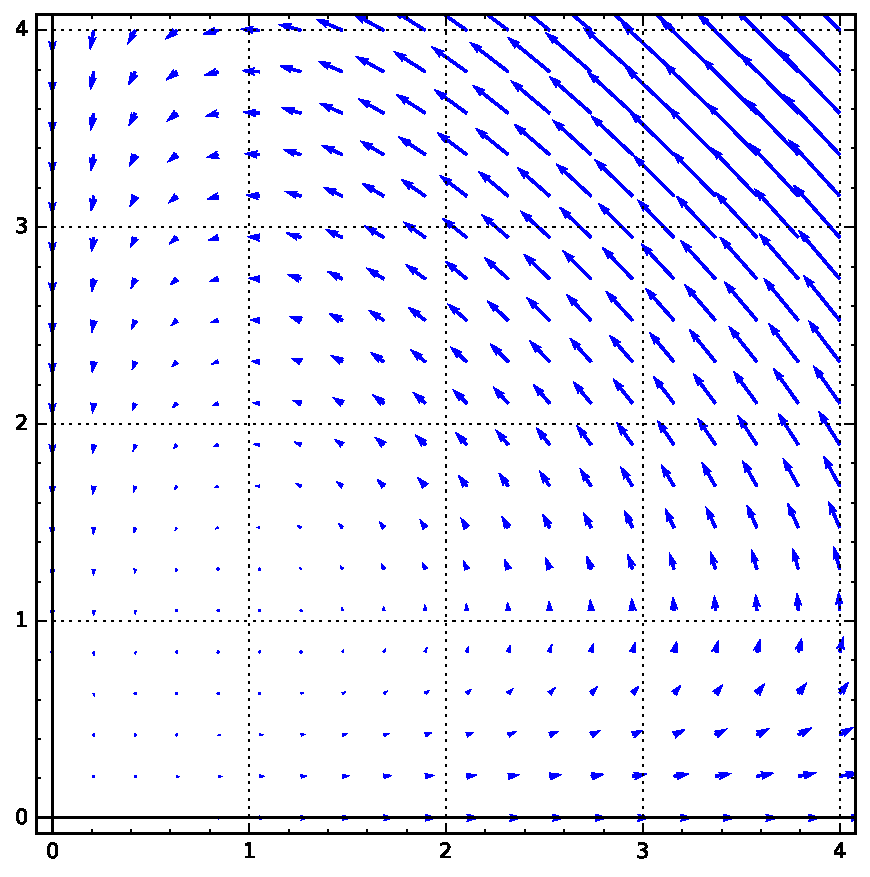
\includegraphics[width=0.46\textwidth]{2s_phase_plane}}}%
\quad
\subfloat[Normalized phase plane]{
    {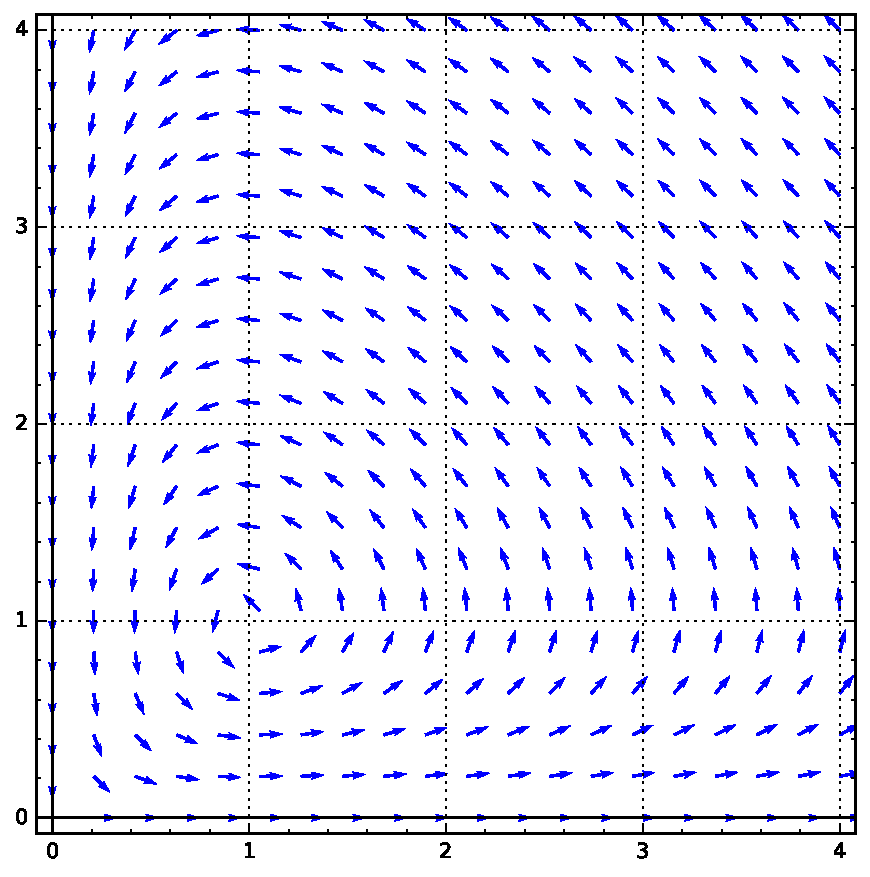
\includegraphics[width=0.46\textwidth]{2s_phase_plane_normalized}}}%
\captionsetup{justification=centering}
\caption{Two-species system phase planes with $a=b=c=d=1$}%
\label{fig:2s_phase_plane}%
\end{figure}
\end{frame}

\begin{frame}{Phase Plane with Contours}
\begin{equation}
    C = a \ln y - by + c \ln x - dx
\label{eq:2s_solution}
\end{equation}
\makefig{H}{0.6\textheight}{2s_phase_plane_contours}{Two-species system phase plane with normalized vectors, contour lines, and $a=b=c=d=1$}
\end{frame}

\begin{frame}{Case $x=0$}
\makefig{H}{0.85\textwidth}{2s_x_zero_graph}{Two-species system graph for $x=0$, $y=3$, and $a=b=c=d=1$}
\end{frame}

\begin{frame}{Case $y=0$}
\makefig{h}{0.8\textwidth}{2s_y_zero_graph}{Two-species system graph for $x=6$, $y=0$, and $a=b=c=d=1$}
\end{frame}

\begin{frame}{Case $x=6$, $y=3$ Contour}
\makefig{h}{0.65\textwidth}{2s_contour}{Two-species system contour for $x=6$, $y=3$, and $a=b=c=d=1$}
\end{frame}

\begin{frame}{Case $x=6$, $y=3$ Graph}
\makefig{h}{0.8\textwidth}{2s_graph}{Two-species system graph for $x=6$, $y=3$, and $a=b=c=d=1$}
\end{frame}

%==============================================================================

\section{Three-Species Food Chain}

\begin{frame}{Three-Species Food Chain}
\begin{itemize}
\setlength\itemsep{1em}
    \item equation \eqref{eq:3s_system} with simple parameters
    \item $a=b=c=d=e=f=g=1$ makes the system
\end{itemize}
\begin{equation}
    \left\{\begin{aligned}
        &\frac{dx}{dt} = x(1 - y)              &\text{Prey}\\
        &\frac{dy}{dt} = y(x - z - 1) \qquad &\text{Intermediate Predator}\\
        &\frac{dz}{dt} = z(y - 1)             &\text{Apex Predator}
    \end{aligned}\right.
    \label{eq:3s_example}
\end{equation}
\end{frame}

\begin{frame}{Case $z=0$}
Equation becomes the same as two-species system
\begin{equation}\nonumber
    \left\{\begin{aligned}
        &\frac{dx}{dt} = x(1 - y)              &\text{Prey}\\
        &\frac{dy}{dt} = y(x - 0 - 1) = y(x-1) 
            \qquad &\text{Intermediate Predator}\\
        &\frac{dz}{dt} = 0(y - 1) = 0             &\text{Apex Predator}
    \end{aligned}\right.
\end{equation}
\end{frame}

\begin{frame}{Case $z=0$ Contour}
\makefig{h}{0.7\textwidth}{3s_z_zero_contour}{Three-species system contour for $x=6$, $y=3$, $z=0$, $a=b=c=d=e=f=g=1$}
\end{frame}

\begin{frame}{Case $z=0$ Graph}
\makefig{h}{0.8\textwidth}{3s_z_zero_graph}{Three-species system graph for $x=6$, $y=3$, $z=0$, $a=b=c=d=e=f=g=1$}
\end{frame}

\begin{frame}{Case $x=0$}
If $x=0$ we get the following equations
\begin{equation}\nonumber
    \left\{\begin{aligned}
        &\frac{dx}{dt} = 0(1 - y) = 0              &\text{Prey}\\
        &\frac{dy}{dt} = y(0 - z - 1)=y(-z-1) 
            \quad &\text{Intermediate Predator}\\
        &\frac{dz}{dt} = z(y - 1)             &\text{Apex Predator}
    \end{aligned}\right.
\end{equation}
\end{frame}

\begin{frame}{Case $x=0$ Graph}
\makefig{h}{0.9\textwidth}{3s_x_zero_graph}{Three-species system graph for $x=0$, $y=3$, $z=1$, $a=b=c=d=e=f=g=1$}
\end{frame}

\begin{frame}{Case $y=0$}
If $y=0$ we get the following system of equations
\begin{equation}\nonumber
    \left\{\begin{aligned}
        &\frac{dx}{dt} = x(1 - 0) = x              &\text{Prey}\\
        &\frac{dy}{dt} = 0(x - z - 1)=0 \qquad &\text{Intermediate Predator}\\
        &\frac{dz}{dt} = z(0 - 1) = -z             &\text{Apex Predator}
    \end{aligned}\right.
\end{equation}
\end{frame}

\begin{frame}{Case $y=0$ Graph}
\makefig{h}{0.9\textwidth}{3s_y_zero_graph}{Three-species system graph for $x=6$, $y=0$, $z=1$, $a=b=c=d=e=f=g=1$}
\end{frame}

\begin{frame}{Further Analysis; Case $ga>fb$}
\begin{itemize}
\setlength\itemsep{1em}
    \item in \cite{chauvet} the authors use further criteria to
        classify \eqref{eq:3s_system}
\begin{equation}\nonumber
    ga > fb, \qquad ga < gb, \qquad  ga = fb.
\end{equation}
\item For example $a=g=1.1$ and all other constants 1
\end{itemize}
\begin{equation}\nonumber
    \left\{\begin{aligned}
        &\frac{dx}{dt} = 1.1x - xy              &\text{Prey,}\\
        &\frac{dy}{dt} = -y + xy - yz \quad &\text{Intermediate Predator,}\\
        &\frac{dz}{dt} = -z + 1.1yz             &\text{Apex Predator.}
    \end{aligned}\right.
\end{equation}
\end{frame}

\begin{frame}{Case $ga>fb$ Graph}
\makefig{h}{0.9\textwidth}{3s_ga_g_fb_graph}{Three-species system graph for $x=6$, $y=3$, $z=1$, $b=c=d=e=f=1$, and $a=g=1.1$}
\end{frame}

\begin{frame}{Case $ga < fb$}
For example $b=f=1.1$ and all other constants equal 1
\begin{equation}\nonumber
    \left\{\begin{aligned}
        &\frac{dx}{dt} = x - 1.1xy              &\text{Prey,}\\
        &\frac{dy}{dt} = -y + xy - yz \quad &\text{Intermediate Predator,}\\
        &\frac{dz}{dt} = -1.1z + yz             &\text{Apex Predator.}
    \end{aligned}\right.
\end{equation}
\end{frame}

\begin{frame}{Case $ga < fb$ Graph}
\makefig{h}{0.9\textwidth}{3s_ga_l_fb_graph}{Three-species system graph for $x=6$, $y=3$, $z=1$, $a=c=d=e=g=1$, and $b=f=1.1$}
\end{frame}

\begin{frame}{Case $ga < fb$ Contour}
\makefig{h}{0.65\textwidth}{3s_ga_l_fb_contour}{Three-species system contour for
$x=6$, $y=3$, $z=1$, $a=c=d=e=g=1$, and $b=f=1.1$}
\end{frame}

\begin{frame}{Case $ga=fb$}
\begin{itemize}
\setlength\itemsep{1em}
    \item original equation \eqref{eq:3s_example} does not change
    \item all constants equal 1, $a=b=c=d=e=f=g=1$
    \item system could be periodic
\end{itemize}
\end{frame}

\begin{frame}{Case $ga=fb$ Graph}
\makefig{h}{0.9\textwidth}{3s_ga_eq_fb_graph}{Three-species system graph for
$x=6$, $y=3$, $z=1$, and $a=b=c=d=e=f=g=1$}
\end{frame}

\begin{frame}{Case $ga=fb$ Contour}
\makefig{h}{0.65\textwidth}{3s_ga_eq_fb_contour}{Three-species system contour for
$x=6$, $y=3$, $z=1$, and $a=b=c=d=e=f=g=1$}
\end{frame}

%==============================================================================

\section{Conclusion}

\begin{frame}{Conclusion}
\begin{itemize}
\setlength\itemsep{1em}
    \item models fit general intuition
    \item inaccuracies: unlimited growth, only one species as prey
    \item equation had great impact on ecology \cite{wangersky}
    \item Lotka-Volterra equations \eqref{eq:2s_system} are among the most
        famous differential equations
\end{itemize}
\end{frame}

\section{Q and A}

\begin{frame}{References}
\begin{thebibliography}{6}
\scriptsize

\bibitem{chauvet}  \textsc{E. Chauvet, J. E. Paullet, J. P. Previte, and Z.
    Walls}, \textit{Lotka-Volterra three-species food chain}, Mathematics
    Magazine, 75 (2002), pp. 243–255. Retrieved from:
    \url{http://www.jstor.org/stable/3219158}.

\bibitem{hoppensteadt}  \textsc{F. Hoppensteadt}, \textit{Predator-prey model},
    Scholarpedia, 1 (2006), p. 1563. Retrieved from:
    \url{http://www.scholarpedia.org/article/Predator-prey_model}.

\bibitem{israel}  \textsc{G. Israel}, \textit{On the contribution of Volterra
    and Lotka to the development of modern biomathematics}, History and
    Philosophy of the Life Sciences, 10 (1988), pp. 37–49. Retrieved from:
    \url{http://www.jstor.org/stable/23328998}.

\bibitem{kreyszig}  \textsc{E. Kreyszig}, \textit{Advanced Engineering
    Mathematics}, John Wiley \& Sons, Inc., 10 ed., 2011.

\bibitem{terman}  \textsc{D. H. Terman and E. M. Izhikevich}, \textit{State
    space}, Scholarpedia, 3 (2008), p. 1924. Retrieved from:
    \url{http://www.scholarpedia.org/article/Phase_space}.

\bibitem{wangersky}  \textsc{P. J. Wangersky}, \textit{Lotka-Volterra
    population models}, Annual Review of Ecology and Systematics, 9 (1978), pp.
    189–218. Retrieved from: \url{https://www.jstor.org/stable/2096748}.

\end{thebibliography}
\end{frame}

\end{document}
